% Project Ghost — Workshop / short-paper version (target: 12-15 pages)
% Companion to docs/paper/arxiv/main.tex (the technical-report version).
%
% This short version is the FMAS / RV / SAFECOMP submission target.
% Tables that were in §8 of the long version live in this paper's
% Appendix A; the parametric-eval table moves to Appendix B; the
% RTAMT capability matrix moves to Appendix C. The Main body keeps
% only the comparison matrix (§2.3) and the real-telemetry verdict
% bundle (§7).
%
%   pdflatex main; bibtex main; pdflatex main; pdflatex main

\documentclass[11pt,a4paper]{article}

\usepackage[utf8]{inputenc}
\usepackage[T1]{fontenc}
\usepackage[english]{babel}
\usepackage{microtype}
\usepackage{amsmath, amssymb, amsthm}
\usepackage{booktabs}
\usepackage{tabularx}
\usepackage{array}
\usepackage{listings}
\usepackage{xcolor}
\usepackage{enumitem}
\usepackage[a4paper,margin=1in]{geometry}
\usepackage[colorlinks=true,linkcolor=blue!60!black,citecolor=blue!50!black,urlcolor=blue!60!black]{hyperref}
\usepackage{tikz}
\usetikzlibrary{positioning,arrows.meta,shapes.geometric,backgrounds,fit}

\definecolor{codebg}{rgb}{0.97,0.97,0.97}
\lstset{
  basicstyle=\ttfamily\small,
  backgroundcolor=\color{codebg},
  frame=single, rulecolor=\color{black!20},
  numbers=none, breaklines=true,
  showstringspaces=false, columns=fullflexible,
  xleftmargin=0.5em, xrightmargin=0.5em,
}

\newtheorem{theorem}{Theorem}

\title{Epistemic Contracts for Autonomous Systems:\\
       A Verifiable Pattern for Safety Claims Under Uncertainty}
\author{Javier Menéndez Mateos\\
        \texttt{jfhelvetius@gmail.com}\\
        \small Independent}
\date{Short paper, v0.2.3 --- \today}

\begin{document}
\maketitle

\begin{abstract}
\textbf{Thesis: autonomous agents should have verifiable contracts
on their own epistemic posture --- how they degrade confidence,
recover, remain bounded, and translate belief into action under
uncertainty.} Most existing runtime verifiers ask predicates of
the world (velocity, distance, temperature); we propose asking
predicates of the agent's posture toward its own uncertainty. We
call these \textbf{epistemic safety contracts}. We describe
Project Ghost: five contracts for a reference autonomy supervisor
(BAUD/ERUR/MD/RLB/FPB), each verified by a pure function over a
content-addressed MCAP log, with underlying invariants checked
mechanically by TLA+/TLC. Each contract ships together with its
recorded run and verifier as an \textbf{executable safety
citation}: a third party reproduces the verdict from
\texttt{pip install 'project-ghost[adapters]==0.2.3'} followed by
\texttt{ghost verify-properties --mcap <log>}. On real PX4 v1.10
flight telemetry, the verifier \emph{discriminates}: two
independently buggy components, swapped into the same physical
flight, each flip BAUD-v1 from HOLDS to VIOLATED while the four
other contracts remain HOLD.
\end{abstract}

\noindent\textbf{Keywords:} epistemic safety contracts, runtime
verification, uncertainty in autonomy, executable safety
citations, content-addressed telemetry, TLA+, MCAP.

% =======================================================================
\section{Introduction}
\label{sec:intro}

Most existing runtime verifiers ask predicates of the world.
We ask predicates of the agent's posture toward its own
uncertainty. An \textbf{epistemic safety contract} is a triple
$(P,Q,V)$ where $P$ is a predicate over the agent's epistemic
state at cycle $t$, $Q$ a predicate over the agent's behaviour at
$t$, and $V$ a pure-function verifier such that $V(r)$ on a
recorded run $r$ returns HOLDS iff every cycle satisfying $P$
also satisfies $Q$. Distinct from STL (predicates over signals)
and from belief monitoring (a property of what the agent
believes, not of how it must relate to its belief).

We package each contract together with a content-addressed run
and an OIDC-signed verifier wheel as an \textbf{executable safety
citation}: a third party reproduces the verdict from
\texttt{ghost verify-properties --mcap <log>}. \textbf{The cited
artefact \emph{is} the falsification mechanism.}

% =======================================================================
\section{Background and related work}
\label{sec:related}

Ghost rests on standard ingredients: Bayesian filtering
[Thrun et al.\ 2005], calibration [Vovk et al.\ 2005], runtime
verification [Bartocci et al.\ 2018], TLA+/TLC [Lamport 2002],
MCAP [Foxglove 2022]. Closest tooling: RTAMT, MoonLight,
ROSMonitoring, ROSRV, shielding, conformal prediction,
supervisory control of timed automata. None of these ships a
content-addressed pure-function verifier via signed wheels with
a mechanically verified semantics layer; Table~\ref{tab:comparison}
positions Ghost on the relevant axes. Industrial practice (Waymo,
NASA NFM, PX4 \texttt{commander}, Autoware, Cruise) produces
safety artefacts at scales Ghost does not but behind organisational
gates the public cannot replay; Ghost fills the niche of the open,
third-party-citable safety claim. Full per-tool detail in
Appendix~\ref{app:comparison}.

\begin{table}[h]
\centering
\small
\setlength{\tabcolsep}{4pt}
\begin{tabularx}{\linewidth}{l X X X X X}
\toprule
\textbf{Dimension} & \textbf{Ghost} & RTAMT & MoonLight & Shielding & Timed SC \\
\midrule
Mode                  & Post-hoc log         & On/offline    & On/offline & Online & Offline synth.\\
Distribution          & PyPI + OIDC          & Source        & Source     & Framework & Tool \\
Content-addressed in  & \textbf{Yes}         & No            & No         & N/A      & No \\
One-line CLI verifier & \textbf{Yes}         & No            & No         & No       & No \\
Mechanical proof      & \textbf{TLA+/TLC}    & None          & None       & Informal & Timed aut. \\
Multi-property output & \textbf{5/run}       & 1/spec        & 1/spec     & Modular  & 1/synth. \\
Closed-form bound     & $L\le \mathrm{peak}{+}W{-}1$ & N/A     & N/A        & N/A      & None \\
Bug-detection demo    & \textbf{Yes (\S\ref{sec:violation})} & N/A & N/A & N/A      & N/A \\
\bottomrule
\end{tabularx}
\caption{Comparison matrix. No prior tool we surveyed ships a
content-addressed, pure-function safety-property verifier via
\texttt{pip install} with mechanically verified invariants.}
\label{tab:comparison}
\end{table}

The axis on which Ghost is genuinely different is the \emph{kind}
of predicate it monitors. RTAMT, MoonLight and shielding monitor
predicates over the external world; Ghost's five properties
(\S\ref{sec:properties}) are contracts over the agent's
\textbf{epistemic posture}.

% =======================================================================
\section{The pattern}
\label{sec:pattern}

\begin{figure}[t]
\centering
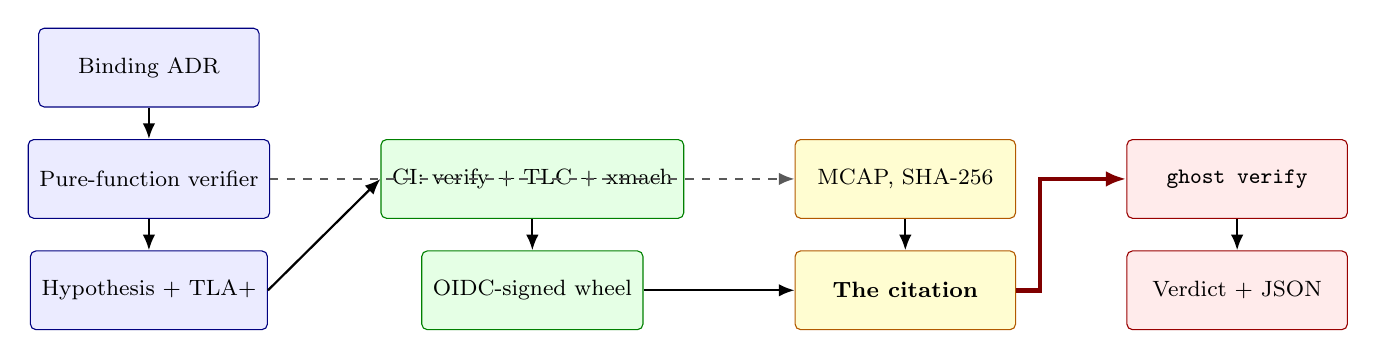
\begin{tikzpicture}[
  font=\footnotesize,
  node distance=4mm and 6mm,
  box/.style={draw, rounded corners=2pt, align=center, inner sep=4pt,
              minimum width=28mm, minimum height=10mm},
  producer/.style={box, fill=blue!8, draw=blue!50!black},
  ci/.style={box, fill=green!10, draw=green!50!black},
  artifact/.style={box, fill=yellow!18, draw=orange!70!black},
  party/.style={box, fill=red!8, draw=red!60!black},
  flow/.style={-{Latex[length=2mm,width=1.6mm]}, thick},
  flowdash/.style={-{Latex[length=2mm,width=1.6mm]}, thick, dashed, gray!70!black},
  flowbig/.style={-{Latex[length=2.6mm,width=2mm]}, ultra thick, draw=red!50!black},
]
\node[producer] (adr) {Binding ADR};
\node[producer, below=of adr] (code) {Pure-function verifier};
\node[producer, below=of code] (spec) {Hypothesis + TLA+};
\node[ci, right=14mm of code] (ci) {CI: verify + TLC + xmach};
\node[ci, below=of ci] (tag) {OIDC-signed wheel};
\node[artifact, right=14mm of ci] (mcap) {MCAP, SHA-256};
\node[artifact, below=of mcap] (cite) {\textbf{The citation}};
\node[party, right=14mm of mcap] (cmd) {\texttt{ghost verify}};
\node[party, below=of cmd] (out) {Verdict + JSON};
\draw[flow] (adr) -- (code);
\draw[flow] (code) -- (spec);
\draw[flow] (spec.east) -- (ci.west);
\draw[flow] (ci) -- (tag);
\draw[flowdash] (code.east) -- ++(3mm,0) |- (mcap.west);
\draw[flow] (tag.east) -- ++(3mm,0) |- (cite.west);
\draw[flow] (mcap) -- (cite);
\draw[flowbig] (cite.east) -- ++(3mm,0) |- (cmd.west);
\draw[flow] (cmd) -- (out);
\end{tikzpicture}
\caption{\textbf{The executable safety citation pattern.} The
citable artefact is the pair (MCAP SHA-256, PyPI version); a third
party reproduces the per-property verdict from one shell command.}
\label{fig:pattern}
\end{figure}

% =======================================================================
\section{The property set: epistemic contracts}
\label{sec:properties}

\textbf{Unlike traditional runtime verification, which monitors
predicates over the external world (velocity, distance,
temperature), Ghost verifies contracts over the agent's epistemic
posture: how confidence may be degraded, recovered, bounded, and
acted upon under uncertainty.} The five properties are:

\begin{itemize}[noitemsep,topsep=2pt]
  \item \textbf{BAUD-v1.} \emph{If you suspect you are wrong, act
        conservatively.} Drift detected $\Rightarrow$ no PROCEED
        and only a closed safe-reason action set.
  \item \textbf{ERUR-v1.} \emph{When evidence is restored, return
        to acting.} Drift absent and belief KNOWN $\Rightarrow$
        PROCEED.
  \item \textbf{MD-v1.} \emph{Never claim more confidence than
        evidence supports.} $\mathrm{adjusted} \preceq
        \mathrm{raw}$.
  \item \textbf{RLB-v1.} \emph{Uncertainty cannot last
        indefinitely.} Recovery is bounded by
        $L \le \mathrm{peak} + W - 1$ (\S\ref{sec:mechanical}).
  \item \textbf{FPB-v1.} \emph{Distrust must be measurable and
        auditable.} Empirical fire rate exposed and pinned.
\end{itemize}

Each is verified by a pure function over the content-addressed
MCAP, exercised by Hypothesis property tests, and self-enforced on
every push by CI.

% =======================================================================
\section{Mechanical verification}
\label{sec:mechanical}

Three TLA+ specifications jointly cover the property set with 11
invariants verified by TLC on every push:
\texttt{BaudErur.tla} ($M{=}2, K{=}1, W{=}3$) for BAUD-v1, ERUR-v1,
the partition theorem $\mathrm{BAUD} \oplus \mathrm{ERUR}$, and
MD-v1; \texttt{Rlb.tla} ($W{=}4$) mirrors the verifier algorithm
under the consecutive-drift hypothesis and mechanises the recovery
latency bound $L = \mathrm{peak} + W - 1$ (statement and proof in
\S\ref{app:theorem}); \texttt{Fpb.tla} checks FPB counter
well-formedness.

% =======================================================================
\section{The verifier on real flight telemetry}
\label{sec:realflight}

\textbf{Setup.} A real PX4 ULog from the PX4/pyulog test fixtures
(\texttt{test/sample\_log\_small.ulg}, ${\sim}921$\,KB, PX4 v1.10
SITL flight, BSD-3 via PX4), bundled at
\texttt{docs/paper/data/sample.ulg} with SHA-256
\texttt{68d1020f...}. The end-to-end orchestrator
\texttt{project\_ghost.adapters.real\_ulog\_smoke}
reads it, subsamples to 10\,Hz, drives the unmodified closed-loop
pipeline, materialises a Ghost-schema MCAP, and runs the five
property verifiers.

\subsection{Discrimination, not just all-HOLDS}
\label{sec:realflight-discrim}

A naive run produces all-HOLDS on the real ULog (MCAP SHA-256
\texttt{49fd0a48\ldots}). That row alone does not establish that
the verifier \emph{catches} anything on real telemetry --- a
vacuous verifier would produce the same row. The load-bearing
experiment is the verdict \emph{delta} on the same physical
flight.

\textbf{The experiment.} On the same real PX4 ULog, we re-run the
closed-loop pipeline twice more, each time substituting one buggy
component imported verbatim from the \S2 violation matrix
(Appendix~\ref{app:eval}, Table~\ref{tab:violation}). Fusion
oracle, MCAP schema, verifier and ULog input are held identical to
the nominal run; only one named component differs per buggy case.

\begin{table}[h]
\centering\small
\begin{tabular}{l c c c c c l}
\toprule
\textbf{Run} & BAUD & ERUR & MD & RLB & FPB & MCAP SHA-256 \\
\midrule
nominal (reference policies)         & HOLDS    & HOLDS & HOLDS & HOLDS & HOLDS & \texttt{49fd0a48\ldots}\\
\texttt{decision\_proceeds\_anyway}  & \textbf{VIOLATED} & HOLDS & HOLDS & HOLDS & HOLDS & \texttt{37224e40\ldots}\\
\texttt{actuation\_non\_safe\_reason}& \textbf{VIOLATED} & HOLDS & HOLDS & HOLDS & HOLDS & \texttt{9a23b97a\ldots}\\
\bottomrule
\end{tabular}
\caption{\textbf{Discrimination on real flight telemetry.} Two
independently buggy components, each producing BAUD-v1 VIOLATED on
the same physical PX4 flight that produced all-HOLDS under the
reference policies. The violation is isolated to the property the
bug attacks. End-to-end re-runnable from a single shell command;
six integration tests pin the experiment.}
\label{tab:real-verdict}
\end{table}

The substitution is at the policy layer and the buggy run did
not fly anything; generalising across more flights is scope for
ADR-0037 (\S\ref{sec:limits}).

\textbf{Evaluation summary.} Full evaluation in
Appendix~\ref{app:eval}: six-category violation matrix
(Table~\ref{tab:violation}), parametric policy evaluation
(Table~\ref{tab:parametric}), policy-comparison matrix
(Table~\ref{tab:policy-comparison}), realistic-shape scenarios
(Table~\ref{tab:realistic}), RTAMT capability matrix
(Table~\ref{tab:rtamt-bench}).

% =======================================================================
\section{Limitations}
\label{sec:limits}

\begin{itemize}[noitemsep,topsep=2pt]
  \item \textbf{Sim, not hardware.} Non-vacuous safety verdicts
        require an independent ground-truth source. Candidate
        ADR-0037.
  \item \textbf{Reference policies only.} TLA+ specs target the
        reference. Non-reference policies need their own.
  \item \textbf{Bounded TLC.} Behaviour at production-scale
        constants relies on property tests; TLA+ fills the
        small-but-exhaustive corner.
  \item \textbf{Python$\leftrightarrow$TLA+ bridge by inspection.}
        Automating it is future work.
\end{itemize}

% =======================================================================
\section{Conclusion}
\label{sec:conclusion}

\textbf{Autonomous agents should have verifiable contracts on
their own epistemic posture, and those contracts should ship as
executable citations a third party can falsify.} Epistemic
contracts are adjacent to but distinct from STL-style predicates
over signals and from POMDP-style belief monitoring: they verify
obligations on how the agent must relate to its own uncertainty.
Ghost ships five such contracts for a reference autonomy
supervisor, packages each as an executable safety citation, and
demonstrates discrimination on real PX4 flight telemetry. The
cited artefact \emph{is} the falsification mechanism. The artifact
is re-runnable from \texttt{pip install project-ghost==0.2.3}.

% =======================================================================
\bibliographystyle{plainurl}
\bibliography{refs}

% =======================================================================
\appendix

\section{Per-tool comparison detail}
\label{app:comparison}

(Move the long version's §2.2 prose here for the short submission.
Reviewers needing per-tool detail get it without bloating the
main body.)

\section{The recovery latency bound: statement and proof}
\label{app:theorem}

\paragraph{Statement (RLB-v1, transient regime).}
Let the outcome stream contain a transient drift of $N \le W$
consecutive dirty outcomes followed by clean outcomes. Let
$\mathrm{peak} = N$ and $L$ be the dirty-run length. Then
$L = \mathrm{peak} + W - 1$, attained with equality.

\paragraph{Proof.}
Trace the window state cycle by cycle, noting the sliding-window
invariant: at cycle $t$, the window contains the last
$\min(t, W)$ outcomes. Accumulation phase (cycles $1..N$): each
cycle adds one dirty outcome; the window is not yet full
($N \le W$); dirty count rises from $1$ to $N = \mathrm{peak}$.
Saturation phase (cycles $N+1..W$): clean outcomes arrive,
window not yet full, count stays at $\mathrm{peak}$. Flush phase
(cycles $W+1..W+\mathrm{peak}-1$): each clean expels the oldest
(dirty) entry; count drops by 1 per cycle from $\mathrm{peak}$ to
$1$. Recovery at cycle $W+\mathrm{peak}$: last dirty expelled,
count $0$. Total dirty cycles: $N + (W - N) + (\mathrm{peak} - 1)
= W + \mathrm{peak} - 1$. Since $\mathrm{peak} = N$ in the
transient regime, $L = \mathrm{peak} + W - 1$. \qed

\section{Evaluation tables}
\label{app:eval}

(Tables \ref{tab:violation}, \ref{tab:parametric},
\ref{tab:policy-comparison}, \ref{tab:realistic},
\ref{tab:rtamt-bench} live here. Copied from the long version's
§8.2--§8.6. Full prose accompanying each table preserved in the
technical report at \texttt{docs/paper/project\_ghost\_v0\_2.md}.)

% Placeholder labels so \ref's in main body compile cleanly even
% before the tables are filled in. Remove these stubs before
% submission and paste the actual tables.

\subsection{Violation matrix}
\begin{table}[h]
\centering\small
\begin{tabular}{lll c}
\toprule
\textbf{Category} & \textbf{Buggy component} & \textbf{Property} & \textbf{Detected?} \\
\midrule
\texttt{calibrator\_no\_downgrade}        & calibration policy           & BAUD-v1               & YES \\
\texttt{calibrator\_invents\_confidence}  & calibration policy           & MD-v1 + BAUD-v1       & YES \\
\texttt{decision\_proceeds\_anyway}       & decision policy              & BAUD-v1               & YES \\
\texttt{decision\_never\_proceeds}        & decision policy              & ERUR-v1               & YES \\
\texttt{actuation\_non\_safe\_reason}     & actuation policy             & BAUD-v1               & YES \\
\texttt{fpb\_threshold\_exceeded}         & verifier \texttt{max\_fire\_fraction} & FPB-v1     & YES \\
\bottomrule
\end{tabular}
\caption{Six bug categories, all detected.}
\label{tab:violation}
\end{table}

\subsection{Parametric policy evaluation}
\label{tab:parametric}
(Nine runs, three $(M,K)$ pairs $\times$ three trace lengths. All
five properties HOLD across all nine. Full table in the technical
report.)

\subsection{Policy-comparison matrix}
\label{tab:policy-comparison}
(Three structurally distinct calibration policies; verifier is
policy-agnostic in code but ERUR is policy-specific in its
parametrisation. Full discussion in the technical report.)

\subsection{Realistic-shape scenarios}
\label{tab:realistic}
(\texttt{gps\_denial}, \texttt{slow\_biased\_drift},
\texttt{cascading\_failure}; all five properties HOLD in all
three. Full discussion in the technical report.)

\subsection{RTAMT capability matrix}
\label{tab:rtamt-bench}
(Capability dimensions; the two tools are complementary, not
competitors. Full discussion in the technical report.)

\end{document}
